\documentclass{article}
\usepackage{amsmath}
\usepackage{graphicx}
\usepackage{caption}
\usepackage{subcaption}
\usepackage{float}


\newcommand{\field}[1]{\item \texttt{ #1 }}

\begin{document}
\title{Homework 1 - Final Writeup}
\author{Patrick Collins}
\date{\today}
\maketitle

\section{Design Changes}
The primary changes to the design resulted from a misunderstanding of
how threads worked. Initially, I thought that, like
ThreadExecutorPools in Python, it was possible to start up one or more
threads and then pass functions and arguments to be executed to each
thread. This was incorrect. Additionally, I was unaware of the
\texttt{pthread\_barrier\_t} construct discussed in class, which I
used to replace the interrupt-based synchronization that I had tried
to implement myself. 

As a result, the \texttt{TSGraph} module became significantly
simpler. The code in the \texttt{hw1/code} directory shows the
changes. Each thread was spawned to execute \texttt{update\_dists\_p},
which divided work across threads along the middle loop index,
\texttt{i}, a call to \texttt{pthread\_barrier\_wait} was added at
the end of each iteration of \texttt{k}, and the \texttt{TSGraph}
object was expanded to have-a \texttt{pthread\_barrier\_t} object. 

The unit testing scheme which attempted to explicitly verify that the
synchronization mechanism I had attempt to implement was working was
abandoned. The use of \texttt{pthread\_barrier\_t} objects for
synchronization obviated the need for unit testing of synchronization,
since they are part of the standard library. 

\section{Hypotheses}
Parallel overhead: \\
It is expected that serial code will run faster
than parallel code for $T = 1$, with the difference between serial and
parallel closing as the size of the input matrix rises. This is
consistent with a small, constant slowdown for spawning a thread, and
identical performance when executing the algorithm.\bigskip

\noindent
Parallel speedup: \\
For input matrix sizes less than 1024 x 1024, it is expected that
there will be two local maxima for performance around  $T = 8$ and $T
= 16$, which represent the maximum number of cores on either one or
both CPUs available on the machine, respectively. The global maximum
is expected to be at $T = 16$. \smallskip

\noindent
Noting that, at 1024 x 1024, the matrix will no longer be able to fit
inside of a single one of the two shared 2 MB L2 caches, it is
expected that while performance will be better than serial, the
improvement will be significantly smaller than on smaller input
matrices. 

\section{Results}
\subsection{Data}
All times are given in milliseconds, with the standard deviation of
each measurement given
in parentheses beside it. The parallel table lists the number of threads above
each column. Each combination of size and number of threads was tested
for 102 runs. The graphs used for input are available in the
\texttt{hw1/input} directory, and the Python script used to generate
the graphs is available under \texttt{hw1/scripts} directory. For
inputs where $T > N$, the number of threads spawned was limited to the
number of nodes, so measurements in these cases are not meaningful.



Serial:
\begin{center}
\begin{tabular}{rl}
 Size  &  Time                 \\
   16  &  0.0208 (0.0072)      \\
   32  &  0.1991 (0.0140)      \\
   64  &  1.5642 (0.0460)      \\
  128  &  11.7189 (0.9526)     \\
  256  &  38.7142 (1.3934)     \\
  512  &  295.5764 (4.0297)    \\
 1024  &  2345.0770 (14.0698)  \\
\end{tabular}
\end{center}


Parallel: 
\begin{center}
\begin{tabular}{rllll}
 Size  &  1                    &  2                    &  4                    &  6                   \\
   16  &  0.4604 (0.0425)      &  0.8946 (0.0586)      &  1.3472 (0.0618)      &  1.8625 (0.0758)     \\
   32  &  0.8311 (0.0358)      &  1.2724 (0.0613)      &  1.5933 (0.0783)      &  2.3739 (0.2274)     \\
   64  &  3.3997 (0.0298)      &  2.9059 (0.1016)      &  2.7252 (0.0565)      &  3.2825 (0.1342)     \\
  128  &  21.4184 (1.7393)     &  13.7050 (0.0790)     &  9.6477 (0.4377)      &  8.5488 (0.1838)     \\
  256  &  80.9646 (2.7891)     &  55.5075 (5.2755)     &  51.1636 (0.3498)     &  38.0607 (1.3370)    \\
  512  &  544.3449 (2.9900)    &  307.2133 (10.4430)   &  181.1431 (11.7229)   &  134.3976 (11.6092)  \\
 1024  &  4276.2213 (12.9687)  &  2184.5808 (23.4179)  &  1167.4299 (38.8022)  &  845.0798 (31.8830)  \\
\end{tabular}
\end{center}


\begin{center}
\begin{tabular}{rllll}
 Size  &  8                   &  16                   &  32                   &  64                   \\
   16  &  2.4409 (0.1161)     &  4.6699 (0.1576)      &  4.6723 (0.2145)      &  4.6327 (0.1338)      \\
   32  &  3.3049 (0.3037)     &  7.6298 (0.2288)      &  15.2066 (0.4301)     &  15.2369 (0.4480)     \\
   64  &  4.3284 (0.3363)     &  13.6072 (0.4845)     &  28.2336 (0.9766)     &  57.2860 (2.4089)     \\
  128  &  9.0134 (0.5320)     &  27.0206 (1.4926)     &  56.7911 (3.7178)     &  113.7569 (5.5547)    \\
  256  &  36.3886 (0.9339)    &  60.6246 (5.8600)     &  124.8831 (9.1391)    &  254.6490 (5.9247)    \\
  512  &  171.4546 (7.0225)   &  231.2499 (25.7973)   &  349.0613 (14.4745)   &  601.3639 (7.8731)    \\
 1024  &  753.5782 (46.1587)  &  575.8449 (215.8510)  &  1557.1865 (15.9205)  &  1904.4370 (34.3756)  \\
\end{tabular}
\end{center}



\begin{figure}[H]
  \centering
  \begin{subfigure}{70mm}
    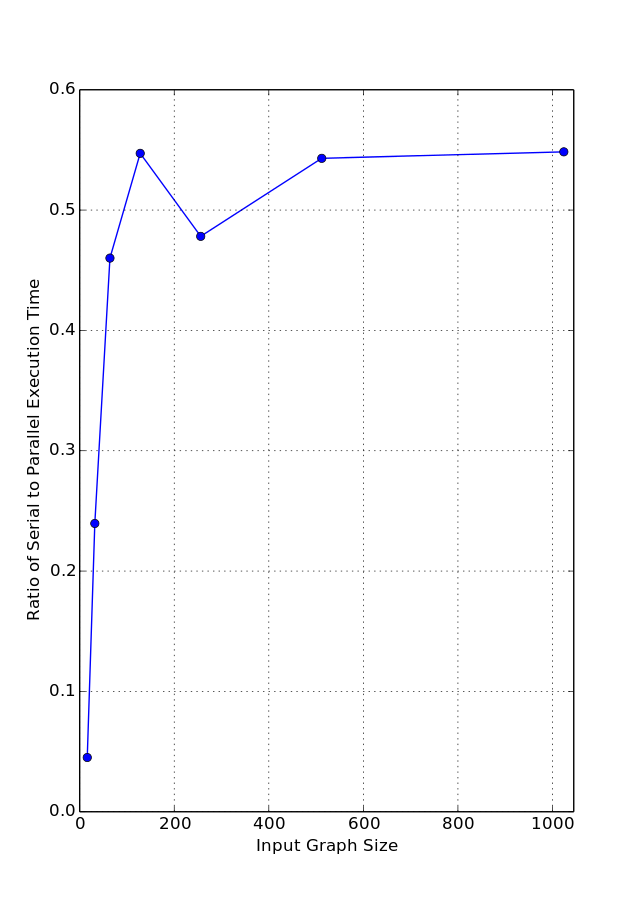
\includegraphics[width=70mm]{./parallel-overhead.png}
    \caption{Parallel Overhead}
  \end{subfigure}
  \begin{subfigure}{60mm}
    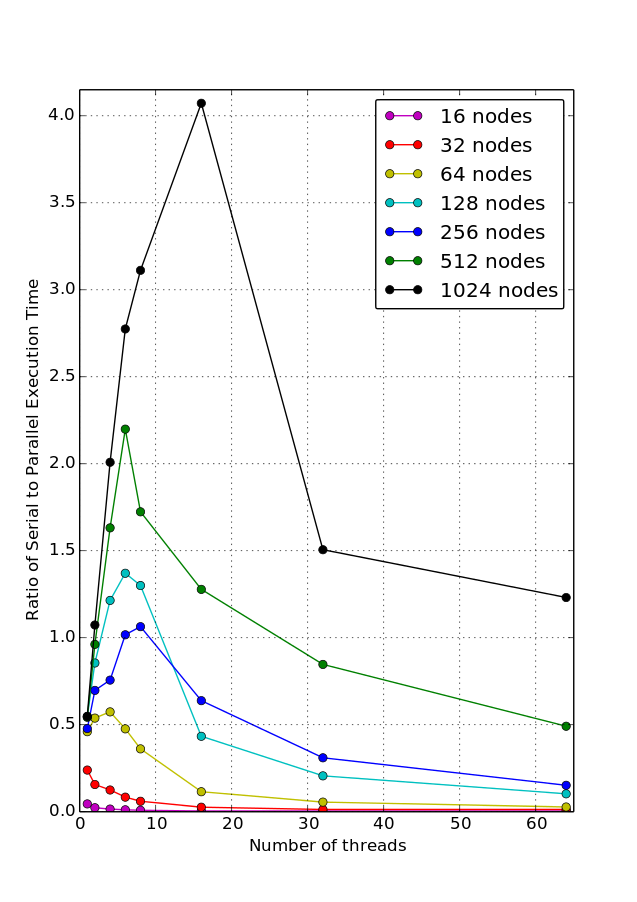
\includegraphics[width=70mm]{./parallel-speedup.png}
    \caption{Parallel Speedup}
  \end{subfigure}
\end{figure}


\pagebreak
\subsection{Analysis}
The hypothesis regarding parallel overhead was disproved. For smaller
graphs, the serial version was as much as 10x faster than the parallel
version running with one thread. Two separate sources of inefficiency
can be identified: first, for smaller graph sizes, the overhead is
likely due to spawning a new thread. For larger graph sizes, it seems
improbable that this would continue to be a significant
factor. Therefore, it is more likely that this slowdown was caused by
the use of
\texttt{pthread\_barrier\_wait} inside of the outer loop of
\texttt{\_update\_dists\_p}. \texttt{pthread\_barrier\_wait} must
include some sort of atomic decrement operation that allows each
thread to update the state of the barrier when it reaches it. This
operation is evidently very expensive, as the parallel code ran at at
most half the speed of the serial code for $T = 1$. 


The first hypothesis regarding parallel speedup was partially confirmed and
partially disproved. The measurements do exhibit maxima at $T = 8$ and
$T = 16$. These maxima, however, are not present within measurements
of a single graph size. Rather, they are present across different
graph sizes: for $N < 1024$, the greatest speedup tends to occur
around 6 or 8 threads, with the maximum occurring closer to 1 for
smaller graph sizes. For $N = 1024$, however, the maximum occurs at $N
= 16$, where a speedup of approximately 4x relative to serial is
achieved. 

The second hypothesis regarding parallel speedup was disproved. It
appears that the benefits of parallelism outweigh any negative effects
on cache locality for $N \leq 1024$.




\end{document}
